%\documentclass[a4paper,doc]{apa6}
\documentclass[a4paper]{article}
% \graphicspath{{/figures/}{./../figures/}}

\usepackage[utf8]{inputenc}
\usepackage[american]{babel}
\usepackage{csquotes}
\usepackage[style=apa,sortcites=true,sorting=nyt,backend=biber]{biblatex}
\addbibresource{referenties.bib}

\usepackage[colorlinks=true, urlcolor=blue, citecolor=blue, linkcolor=blue]{hyperref}

%\usepackage{apacite}
\usepackage{authblk}  % for authors
\usepackage{xcolor}
\definecolor{mypink}{RGB}{255, 230, 255}

\usepackage{nicefrac}
\usepackage{amsmath}
\usepackage{graphicx}
\usepackage{chngcntr} % appendix references
\usepackage[colorinlistoftodos,prependcaption]{todonotes}
\usepackage{pgfplotstable}
\pgfplotstableset{
	fixed zerofill,
	precision=3,
	col sep = comma,
	search path={../tables/}
}
\pgfkeys{/pgf/number format/precision=2, /pgf/number format/fixed}%

\newcommand{\getValue}[3]{%
	\pgfplotstablegetelem{#1}{#2}\of{#3}%
	\pgfmathprintnumber{\pgfplotsretval}%
}
\newcommand{\setValue}[4]{%
	\pgfplotstablegetelem{#1}{#2}\of{#3}%
	\pgfmathprintnumberto{\pgfplotsretval}{#4}%
}


\newcommand{\getCI}[2]{[\getValue{#1}{Lower}{#2}, \getValue{#1}{Upper}{#2}]}

%\usepackage{titlesec}
%
%\titlespacing\section{0pt}{8pt plus 4pt minus 2pt}{4pt plus 2pt minus 2pt}
%\titlespacing\subsection{0pt}{8pt plus 4pt minus 2pt}{0pt plus 2pt minus 2pt}
%\titlespacing\subsubsection{0pt}{8pt plus 4pt minus 2pt}{0pt plus 2pt minus 2pt}

\usepackage{changes}
\usepackage[normalem]{ulem}
\setdeletedmarkup{\color{red}\emph{\sout{#1}}\color{black}}

\usepackage{tikz}
\usepackage{tikzscale} % check if used!

\usepackage[most]{tcolorbox}

\newtcolorbox[auto counter]{NewBox2}[2][]{
	colframe=black,colback=white,
	enhanced,
%	breakable,
	title={Box \thetcbcounter: #2},
	colbacktitle=white,
	coltitle = black,
	detach title,
	before upper={\tcbtitle\quad},
	#1
}
%\getValue{0}{ph0}{\reanalysis}

\usepackage{setspace}
\doublespacing

\newcommand{\EJ}[1]{\todo[inline, color=green]{  #1 }}
\newcommand{\Q}[1]{\todo[inline, color=yellow]{  #1 }}
\newcommand{\jv}[2]{{\color{red}\st{#1}}{\color{blue}\bf{#2}}}
\newcommand{\DON}[1]{\todo[inline, color=white]{Don: #1}}
\newcommand{\DONside}[1]{\todo[color=white]{#1}}
%\newcommand{\DONTODO}[1]{{\color{red}{#1}} \addcontentsline{tdo}{todo}{#1}}
\newcommand{\J}[1]{\todo[inline, color=mypink]{#1}}

\graphicspath{{../figures/}}
\newcommand{\hypo}[1]{\ensuremath{\mathcal{H}_{#1}}}
\newcommand{\shypo}[1]{%
	\ifnum#1>0%
		\mathrm{slab}
	\else%
		\mathrm{spike}
	\fi%
}
\newcommand{\model}{\mathcal{M}}
\newcommand{\data}{\mathrm{data}}%\mathcal{D}}
\newcommand{\midd}{\ensuremath{\,|\,}}
\newcommand{\cohend}{\ensuremath{d}}

\newcommand{\popDelta}{\delta}
\newcommand{\obsDelta}{\hat{\delta}}

\newcommand{\probo}{\mathrm{Pr}}
\newcommand{\prob}[1]{\probo\left(#1\right)}
\newcommand{\AIC}{\mathrm{AIC}}

\newcommand{\osflink}{\url{https://osf.io/uq8st/}}

\newcommand{\CamererReplication}{\url{https://mfr.osf.io/render?url=https://osf.io/fg4d3/?action=download\%26mode=render}}
\newcommand{\manyLabsLink}{\url{https://mfr.osf.io/render?url=https://osf.io/xufw4/?action=download\%26mode=render}}


\newenvironment{revision}{\color{teal}}{\color{black}}

\title{A Cautionary Note on Estimating Effect Size}
%\shorttitle{Estimating Effect Size} 
\renewcommand{\thefootnote}{\fnsymbol{footnote}}
\author[1]{Don van den Bergh%
	\thanks{%
Correspondence concerning this article should be addressed to: Don van den Bergh, University of Amsterdam, Department of Psychological Methods, Nieuwe Achtergracht 129B, 1018VZ Amsterdam, The Netherlands.
E-Mail should be sent to: donvdbergh@hotmail.com.
This work was supported by a Research Talent grant from the
Netherlands Organisation of Scientific Research (NWO) to DvdB and an
Advanced ERC grant 743086 UNIFY to EJW.
}}
\author[1]{Julia M. Haaf}
\author[1,2]{Alexander Ly}
\author[3]{\authorcr Jeffrey N. Rouder} % putt Jeff on a newline to avoid a newline after his first name
\author[1]{Eric-Jan Wagenmakers}
\affil[1]{University of Amsterdam}
\affil[2]{Centrum Wiskunde \& Informatica}
\affil[3]{University of California Irvine}
\date{}
%\affiliation{~}
\renewcommand*{\thefootnote}{\arabic{footnote}}
%
%\threeauthors{Don van den Bergh and Julia M. Haaf and Alexander Ly and Eric-Jan Wagenmakers}{Alexander Ly}{Jeffrey N. Rouder}
%\threeaffiliations{University of Amsterdam}{Centrum Wiskunde \& Informatica}{University of California Irvine}
%\authornote{Correspondence concerning this article should be addressed to: Don van den Bergh, University of Amsterdam, Department of Psychological Methods, Nieuwe Achtergracht 129B, 1018VZ Amsterdam, The Netherlands. E-Mail should be sent to: donvdbergh@hotmail.com.}

\pgfplotstableread{effectSizeExample.csv}\tbEffectSizeExample
\pgfplotstableread{posteriorProbH0.csv}\reanalysis

\begin{document}

%\listoftodos
%\newpage

\maketitle

\begin{abstract}
	An increasingly popular approach to statistical inference is to focus on the estimation of effect size while ignoring the null hypothesis that the effect is absent.
	We demonstrate how this common ``null hypothesis neglect'' may result in effect size estimates that are overly optimistic.
	The overestimation can be avoided by incorporating the plausibility of the null hypothesis into the estimation process through a ``spike-and-slab'' model.
\end{abstract}

Consider the following hypothetical scenario: a colleague from the biology department has just conducted an experiment and approaches you for statistical advice. The analysis yields $p<0.05$ and your colleague believes that this is grounds to reject the null hypothesis. In line with recommendations both old \parencite[e.g.,][]{Grant1962, Loftus1996} and new \parencite[e.g.,][]{harrington2019new, Cumming2014} you convince your colleague that it is better to replace the $p$-value with a point estimate of effect size and a 95\% confidence interval \parencite[but see][]{MoreyEtAl2016CI}. You also manage to convince your colleague to plot the data (see Figure~\ref{fig:descriptivesPlot}). Mindful of the reporting guidelines of the \emph{Psychonomic Society}\footnote{\protect\url{https://www.springer.com/psychology?SGWID=0-10126-6-1390050-0}} and \emph{Psychological Science}\footnote{\url{https://www.psychologicalscience.org/publications/psychological\_science/ps-submissions\#STAT}}, your colleague reports the result as follows: ``Cohen's $\cohend = \getValue{0}{Estimate}{\tbEffectSizeExample}$, CI $= \getCI{0}{\tbEffectSizeExample}$''.


\begin{figure}[!ht]
	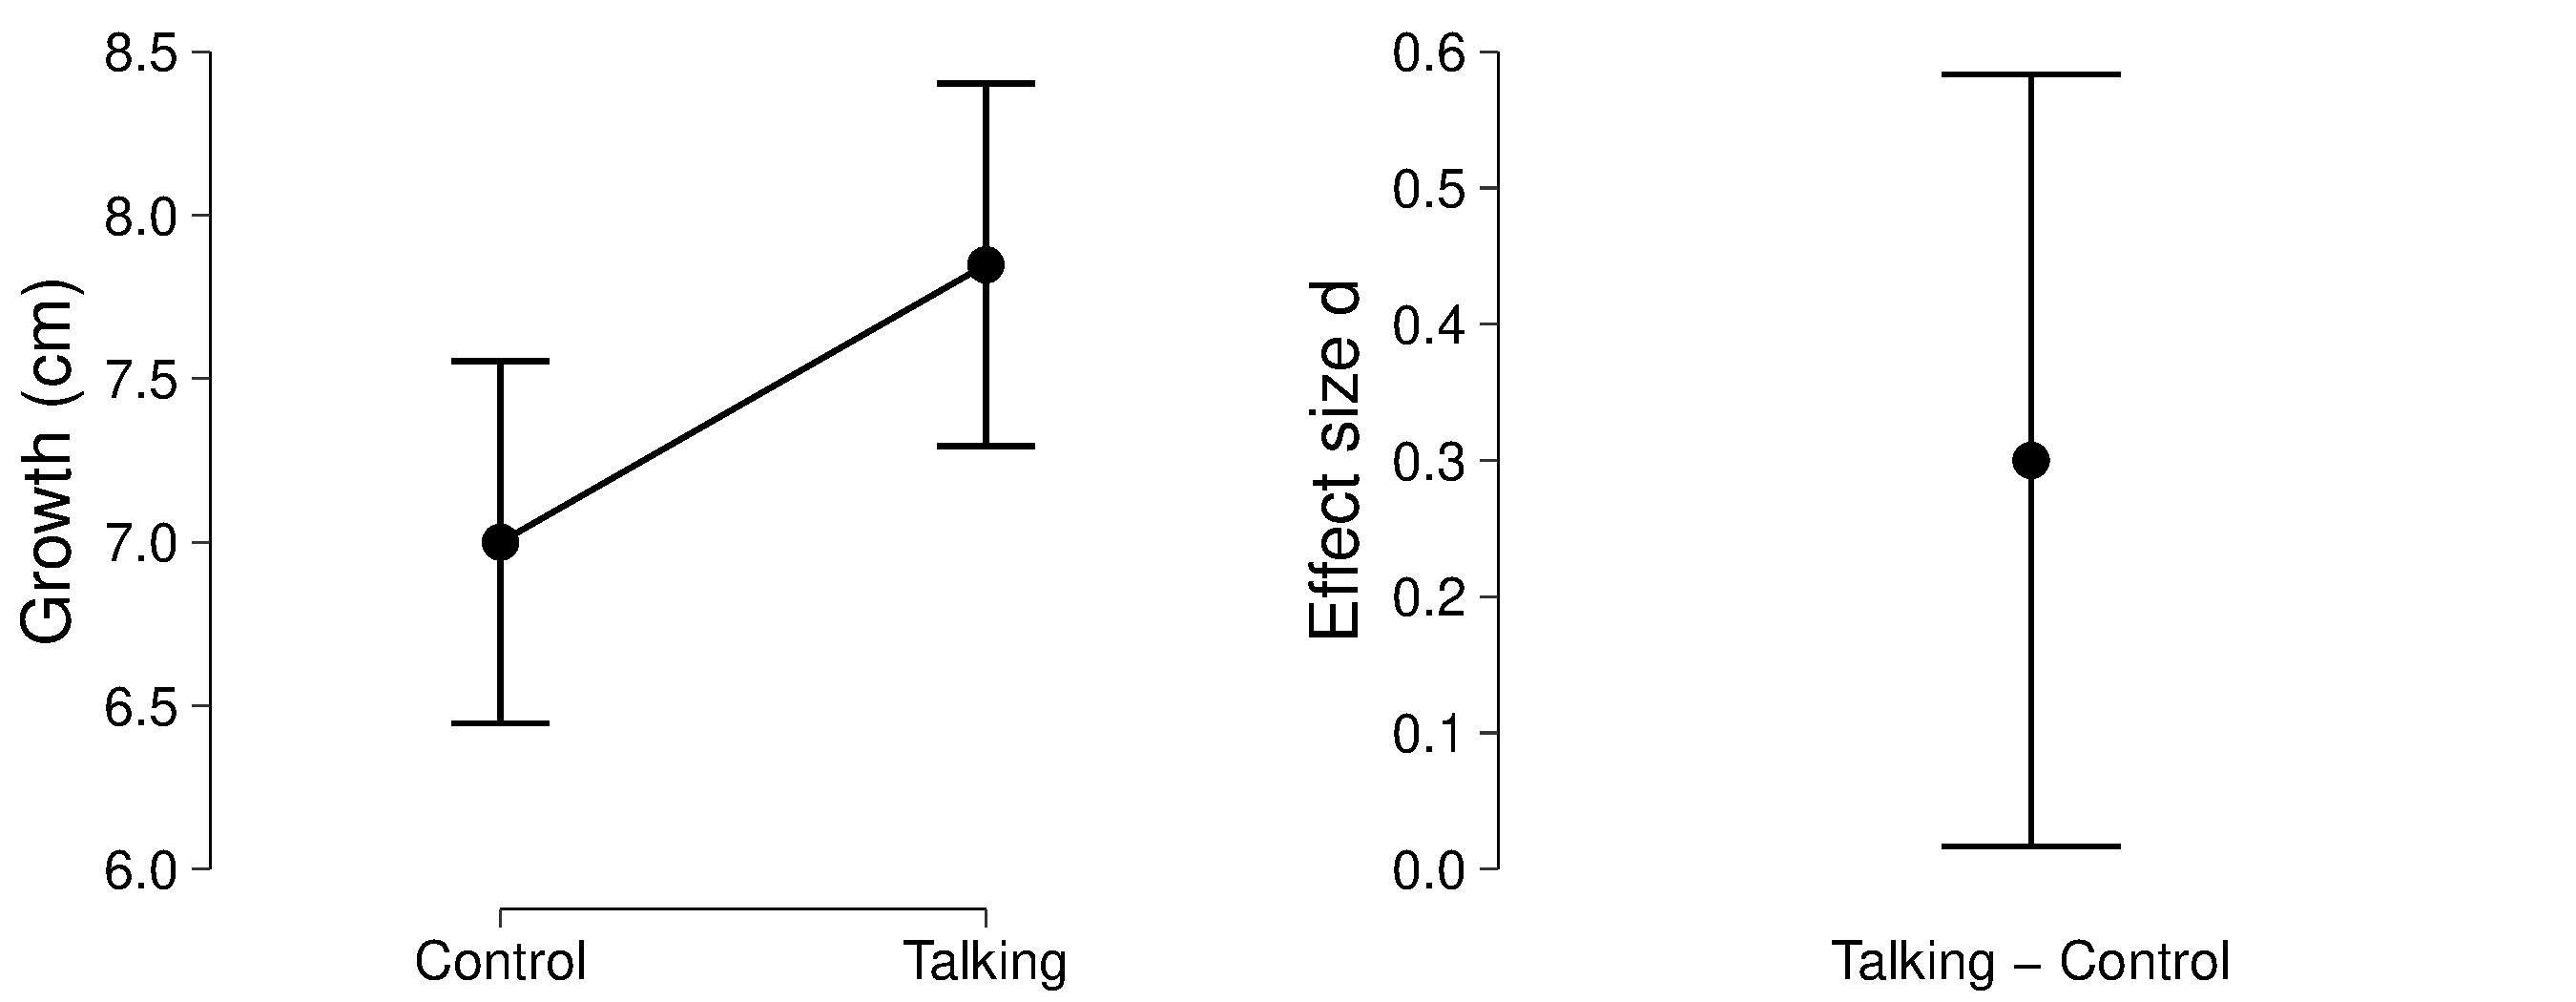
\includegraphics[width=\textwidth]{descriptivesPlot.pdf}
	\caption{Standard estimation results for the fictitious plant growth example. Left panel: a descriptives plot with the mean and 95\% confidence interval of plant growth in the two conditions. Right panel: point estimate and 95\% confidence interval for Cohen's \cohend.}
	\label{fig:descriptivesPlot}
\end{figure}


Based on these results, what would be a reasonable point estimate of effect size? A straightforward and intuitive answer is ``\getValue{0}{Estimate}{\tbEffectSizeExample}''. However, your colleague now informs you of the hypothesis that the experiment was designed to assess: ``plants grow faster when you talk to them''.\footnote{Specifically, imagine your colleague selected 100 plants and weighted them three times: at the start of the experiment, after one week, and after two weeks. The first week 50 plants were randomly selected and spoken to, while the others served as controls. The next week the roles were reversed: the previously spoken to plants served as controls while the control plants were now spoken to. The quantity of interest is the difference in weight between the two conditions. This example is inspired by \protect\textcite{BergerDelampady1987}.} Suddenly, a population effect size of ``0'' appears eminently plausible. Any observed difference may merely be due to the inevitable sampling variability.\footnote{\deleted{Unless your colleague talked out loud, with consumption, and the plants were near.}}

\section*{\deleted{When Are Effect Sizes Overestimated?}}
\begin{revision}%
	The example above raises the question: When are effect sizes overestimated?
\end{revision}%
Standard point estimates and confidence intervals ignore the possibility that the effect is spurious (i.e., the null hypothesis $\mathcal{H}_0$). This is not problematic when $\mathcal{H}_0$ is deeply implausible, either because $\mathcal{H}_0$ was highly unlikely \emph{a priori} or because the data decisively undercut $\mathcal{H}_0$. But when the data fail to undercut $\mathcal{H}_0$, or when $\mathcal{H}_0$ is highly likely \emph{a priori} (i.e., ``plants do not grow faster when you talk to them''), then $\mathcal{H}_0$ is not ruled out as a plausible account of the data. Effect size estimates that ignore a plausible $\mathcal{H}_0$ are generally \begin{revision}biased and\end{revision} overconfident: the fact that $\mathcal{H}_0$ provides an acceptable account of the data should shrink effect size estimates towards zero.

\begin{revision}%
\DON{We could also briefly mention the spike-and-slab model here as a remedy to the problem introduced above.}
\end{revision}%

\begin{revision}%
In this paper, we discuss the spike-and-slab model and its merits to avoid overestimating effect size.
First, we formally introduce the spike-and-slab model.
Second, we apply the spike-and-slab model to the example in the introduction and illustrate how it circumvents overestimation.
Third, we show certain theoretical properties of the spike-and-slab model in a simulation.
Fourth, we demonstrate the spike-and-slab model by reanalyzing the data of \textcite{heycke2018two}.
Finally, we conclude with practical recommendations and a discussion on when not to use the spike-and-slab model.
\end{revision}


\section*{A Spike-and-Slab Perspective}
\begin{revision}%
Here we formalize the conceptual ideas from the introduction in the spike-and-slab model \parencite{RouderEtAl2018PBR, clyde1996prediction, mitchell1988bayesian}. 
%Estimates of effect size, $\obsDelta$, typically assume that \hypo{0} is false and that the population effect size, $\delta$, is nonzero.
The population effect size is typically approximated with a sample estimate.
This sample estimate assumes that \hypo{0} is false and that the population effect size is nonzero.
To formalize this, let $\popDelta$ denote the population effect size, $\obsDelta$ denote it's estimate, and $\obsDelta\mid\hypo{1}$ denotes the estimate that assumes that \hypo{1} is true.
Assuming that \hypo{0} is true, leads to $\obsDelta\mid\hypo{0}$, which is usually 0.
Key is that both estimates, $\obsDelta\mid\hypo{1}$ and $\obsDelta\mid\hypo{0}$, are \emph{conditional} on the hypotheses. 
For example, $\obsDelta\mid\hypo{1}$ should be read as ``the estimated effect size given that the alternative hypothesis is true''.


%Such an estimate is denoted $\obsDelta\mid\hypo{1}$.
%Assuming that \hypo{0} is true, leads to an estimate denoted $\obsDelta\mid\hypo{0}$, which is usually 0. 
%Key is that both estimates, $\obsDelta\mid\hypo{1}$ and $\obsDelta\mid\hypo{0}$, are \emph{conditional} on the hypotheses. 
%For example, $\obsDelta\mid\hypo{1}$ should be read as ``the estimated effect size given that the alternative hypothesis is true''.
%Note that both estimates assume the hypothesis to be true; they ignore any uncertainty regarding the hypotheses themselves.
%The key property of the spike-and-slab model is that it considers both hypotheses at once in a two-component model. 
\end{revision}%
The first component\begin{revision}, the spike, \end{revision}corresponds to the position that talking to plants does not affect their growth (i.e., $\delta = 0$), whereas the second component\begin{revision}, the slab, \end{revision}corresponds to the position that speaking to plants does affect their growth (i.e., $\delta \neq 0$).
\begin{revision}%
\begin{revision}The spike and slab\end{revision} are analogous to \hypo{0} and \hypo{1} discussed above.
\end{revision}%
Both components are deemed \emph{a priori} equally likely, such that the prior probability for each component is \nicefrac{1}{2}.
\begin{revision}%
After seeing the data, the prior probabilities of each component, $\prob{\shypo{0}}$ and $\prob{\shypo{1}}$, are updated to posterior probabilities, $\prob{\shypo{0}\mid\data}$ and $\prob{\shypo{1}\mid\data}$.
Quantifying the uncertainty about the two components using probabilities allows us to account for the uncertainty of each component.
Furthermore, this allows us to consider the \emph{marginal} estimate of effect size.
The marginal estimate of the spike-and-slab model weighs the estimates of each component by its plausibility after seeing the data.
That is, following the law of total probability, we sum the estimates conditional on each component weighed by the posterior probabilities of the components:
\begin{align*}
	\obsDelta = \left(\obsDelta\mid\shypo{0}\right)\prob{\shypo{0}\mid\data} + \left(\obsDelta\mid\shypo{1}\right)\prob{\shypo{1}\mid\data}.
\end{align*}

To obtain the posterior probabilities, we need to choose an inferential paradigm.
In a frequentist approach, one could compute an information criteria for each model, say the Akaike Information Criterion \parencite[AIC;][]{Akaike1973}, and define $\prob{\shypo{0}\mid\data} = \nicefrac{\AIC\mid\shypo{0}}{\left(\AIC\mid\shypo{0} + \AIC\mid\shypo{1}\right)}$.
This approach is taken by, for instance, \textcite{BurnhamAnderson2002}.
An alternative is the Bayesian approach.
Here we assign probability distributions to unknown parameters, such as effect size.
This requires us to specify additional prior distributions, however, the posterior model probabilities follow directly from Bayes theorem and do not depend on the choice of information criteria.
Furthermore, we obtain a posterior distribution for effect size which fully captures the uncertainty over possible effect sizes and allows for easy computation of uncertainty intervals.
In the remainder of this paper, we adopt the Bayesian approach for the spike-and-slab model.
For a full derivation of the posterior distribution, see Appendix A.
\DON{TODO: Actually write this appendix/ box.}
\end{revision}

\begin{revision}To\end{revision} illustrate both the overestimation and \begin{revision}the spike-and-slab model we reanalyze\end{revision} the fictitious data from Figure~\ref{fig:descriptivesPlot}.
\begin{revision}%
	R code for the analysis is available at \osflink{}.
\end{revision}
In almost all current empirical work, an estimate of effect size is based solely on the second component, which yields a point estimate and an uncertainty interval (for frequentists, $\delta = \getValue{0}{Estimate}{\tbEffectSizeExample}$, 95\%  CI: \getCI{0}{\tbEffectSizeExample}; for Bayesians $\delta = \getValue{1}{mean}{\reanalysis}$, 95\% CRI: \getCI{1}{\reanalysis}).
The spike-and-slab model, however, also considers the possibility that an effect can be absent; consequently, the overall estimate from the spike-and-slab model is a weighted average of the two components, shrinking the estimate towards zero.
Figure~\ref{fig:modelAveragedPosterior} contrasts the traditional slab-only estimation against the spike-and-slab estimation.



%Here we illustrate both the overestimation and a remedy by reanalyzing the fictitious data from Figure~\ref{fig:descriptivesPlot}.\footnote{R code for the analysis is available at \osflink{}.} We apply the spike-and-slab model \cite{RouderEtAl2018PBR, clyde1996prediction, mitchell1988bayesian}, which consists of two components. The first component corresponds to the position that talking to plants does not affect their growth (i.e., $\delta = 0$), whereas the second component corresponds to the position that speaking to plants does affect their growth (i.e., $\delta \neq 0$). Both components are deemed \emph{a priori} equally likely, such that the prior probability for each component is \nicefrac{1}{2}. Here we view the spike-and-slab setup as a single model, although it can also be viewed as a form of Bayesian model averaging (see Box~\ref{box:box1} for details). In almost all current empirical work, an estimate of effect size is based solely on the second component, which yields a point estimate and an uncertainty interval (for frequentists, $\delta = \getValue{0}{Estimate}{\tbEffectSizeExample}$, 95\%  CI: \getCI{0}{\tbEffectSizeExample}; for Bayesians $\delta = \getValue{1}{mean}{\reanalysis}$, 95\% CRI: \getCI{1}{\reanalysis}). The spike-and-slab model, however, also considers the possibility that an effect can be absent; consequently, the overall estimate from the spike-and-slab model is a weighted average of the two components, shrinking the estimate towards zero.\footnote{For the spike-and-slab model, the posterior distribution is constructed in the following manner: $p(\delta\midd\data) = 1\{\delta = 0\}\prob{\model_0\midd\data} + p(\delta\midd\data,\model_1)\prob{\model_1\midd\data}$. Here, $1\{\delta = 0\}$ is the Dirac delta function which represents the spike under $\mathcal{H}_0$, $\probo$ denotes probability of a model, and $p$ denotes density related to the magnitude of the effect.} Figure 2 contrasts the traditional slab-only estimation against the spike-and-slab estimation.
% these cannot be generated inside the caption
\setValue{0}{ph1}{\reanalysis}{\phAlt}%
\setValue{0}{mode}{\reanalysis}{\modeAlt}%
\begin{figure}[!ht]
	\centering
	\begin{tikzpicture}
		\node[anchor=south west,inner sep=0] (image) at (0,0) {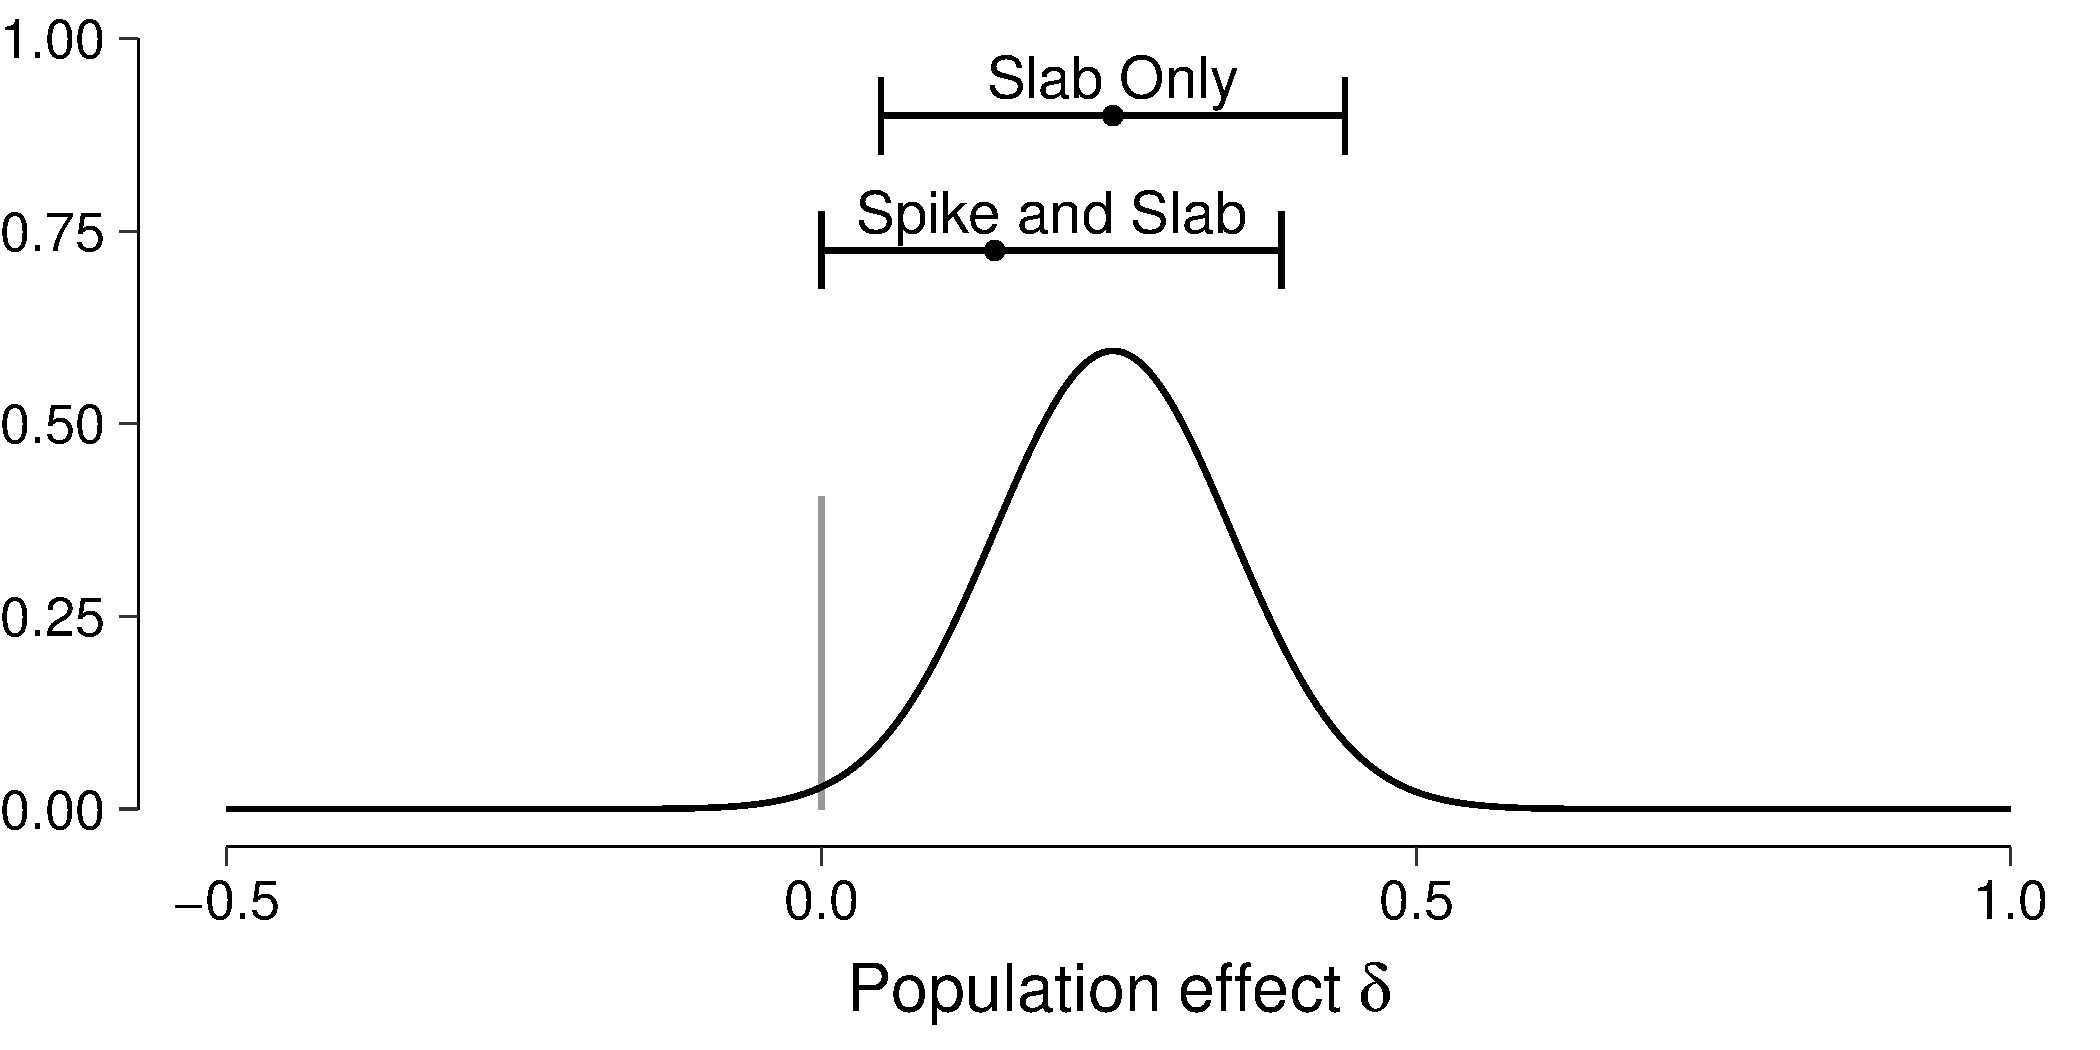
\includegraphics[width=0.9\textwidth]{spikeAndSlabPosteriorRescaledPosteriorMode.pdf}};
		\begin{scope}[x={(image.south east)},y={(image.north west)}]
		\node[anchor=base,inner sep=0pt, outer sep=0pt] at (0.28,0.61) {$p(\hypo{0}\mid\data) = \getValue{0}{ph0}{\reanalysis}$};
		\end{scope}
	\end{tikzpicture}
	\caption{
		The spike-and-slab model. The black line represents the posterior distribution of effect size given the slab (i.e., the effect is non-zero). The posterior is scaled so that its mode ($\delta = \modeAlt$) equals the posterior probability of the alternative model (i.e., $p(\hypo{1}\mid\data) = \phAlt$). The grey line represents the posterior probability of the spike (i.e., $\mathcal{H}_0$: the effect is absent). The error bars and dots above the density show 95\% credible intervals and the posterior mean for the slab-only model and for the spike-and-slab model.}
	\label{fig:modelAveragedPosterior}
\end{figure}
Compared to the traditional results based only on the slab, the posterior mean and central 95\% credible interval of the spike-and-slab model are shrunken towards 0 (i.e., \getValue{0}{mean}{\reanalysis} (95\% CRI: \getCI{0}{\reanalysis}) vs. \getValue{1}{mean}{\reanalysis} (95\% CRI: \getCI{1}{\reanalysis})). This shrinkage is due to the non-negligible probability that the effect is absent. The spike-and-slab posterior represents the plausibility that the effect is absent by the height of the spike, and the uncertainty about the effect's magnitude, given that it is present, by the width of the slab. Note that as the posterior probability of $\mathcal{H}_0$ decreases, the spike-and-slab results approach those of the slab-only model.



\begin{revision}%
%\section*{Simulation results}
\section*{The Influence of the Spike}

In the fictitious example, the spike-and-slab model avoids overestimation by shrinking estimates of effect size towards 0.
That result may not be surprising, as the effect was small.
However, it makes one wonder to what extent the spike-and-slab model helps with estimation.
What differs between a spike only model and the spike-and slab?
Here, we illustrate in a simulation how the estimated effect size shrinks towards 0 as a function of the observed effect size, the prior on effect size, the sample size, and the prior probability of the spike.
We chose these parameters because the posterior distribution only depends on these quantities.

Figure~\ref{fig:S_vs_SS_4_panel} shows the relation between the observed effect size and the estimated effect size for the slab and for the spike-and-slab for 40 observations and 100 observations.
The plots in the right column show that a smaller prior standard deviation induces more shrinkage towards 0, regardless of the sample size.
This makes sense as a small prior standard deviation implies there is more prior mass near the mean of the prior, which is 0.
Comparing the plots between the two columns illustrates the influence of the spike; whenever the observed effect size is near zero, the estimate is shrunken towards zero in the right column but not in the left column.
However, when the observed effect size is far from zero, there is little shrinkage.
%The plots in the right column show that the shrinkage decreases as the sample size increases.
%The spike influences the shrinkage more when the sample size is smaller.
\begin{figure}[!ht]
	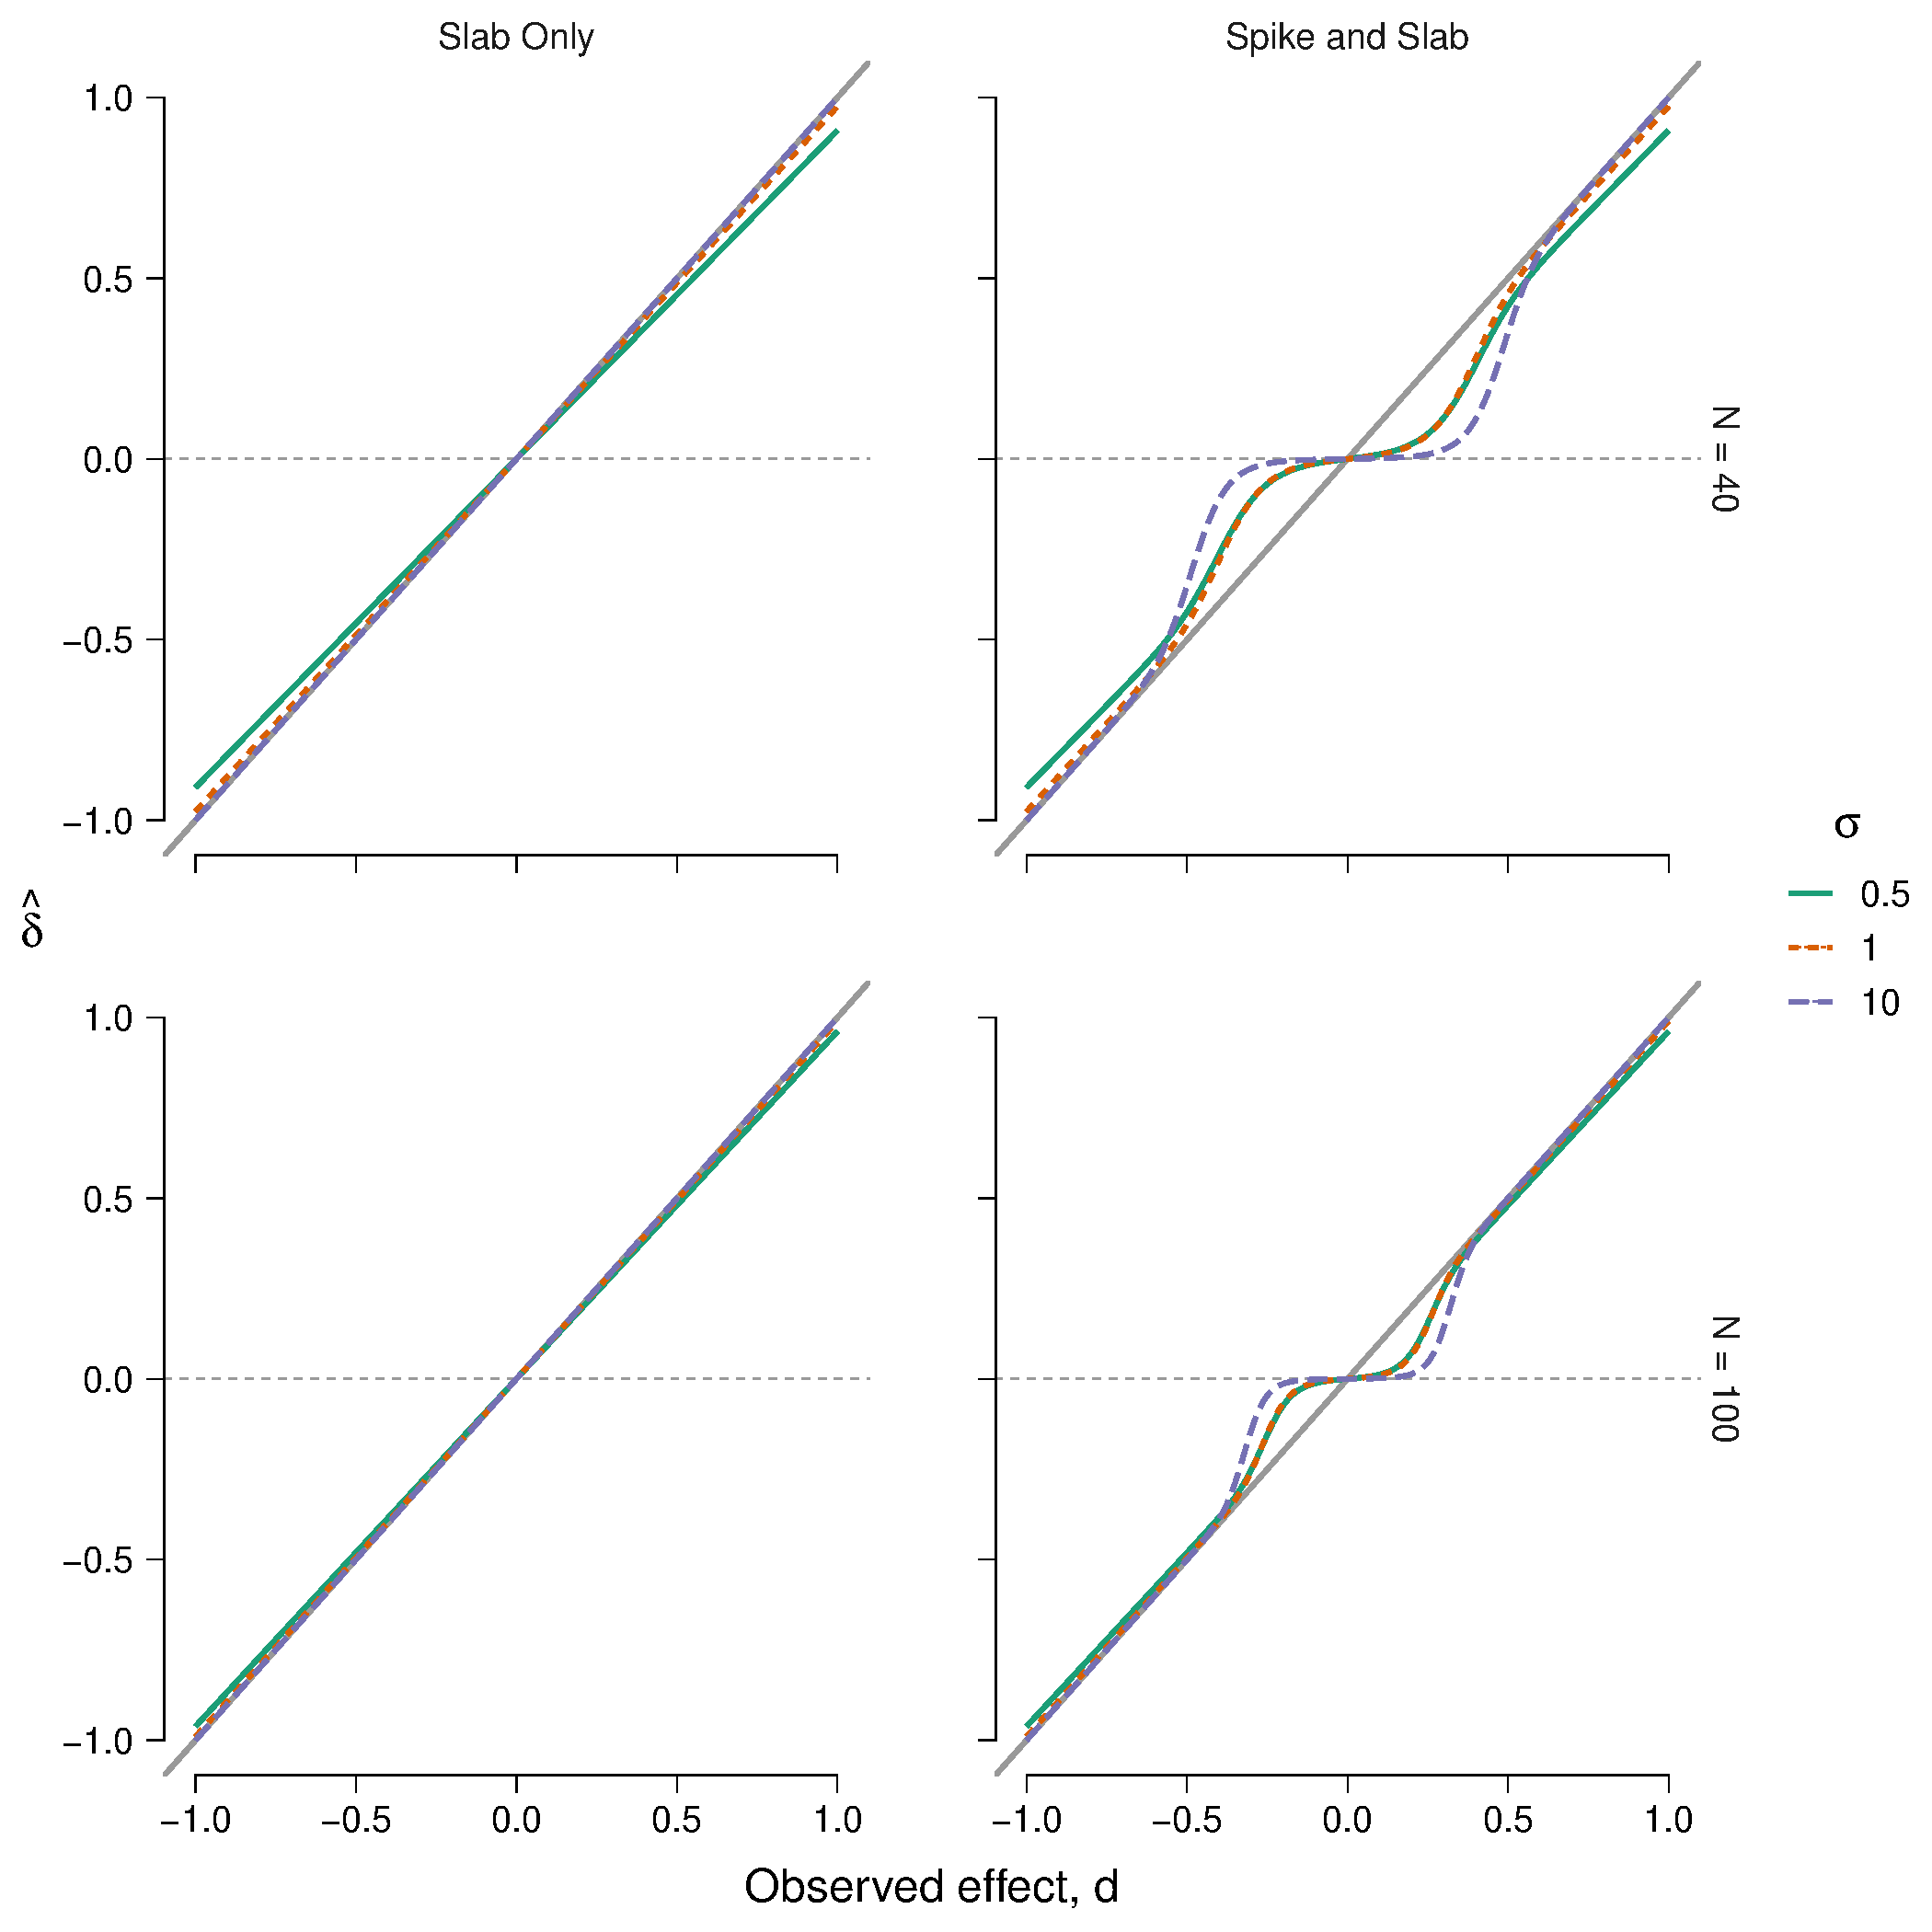
\includegraphics[width=\textwidth]{posteriorMeanVsSampleDelta_4_panel.pdf}
	\caption{%
		Observed effect size versus posterior mean for different model components and prior standard deviations.
		The left column shows inference based on the slab only model while the right column shows inference based on the spike-and-slab model.
		In the top row the sample size was 40 while in the bottom row the sample size was 100.
		Different lines represent different standard deviations for the prior distribution on $\delta$.
		The prior probability of the spike was $\nicefrac{1}{2}$.
		Inspired by Figure~5 of \textcite{RouderEtAl2018PBR}.
	}
	\label{fig:S_vs_SS_4_panel}
\end{figure}
%\begin{figure}[!ht]
%	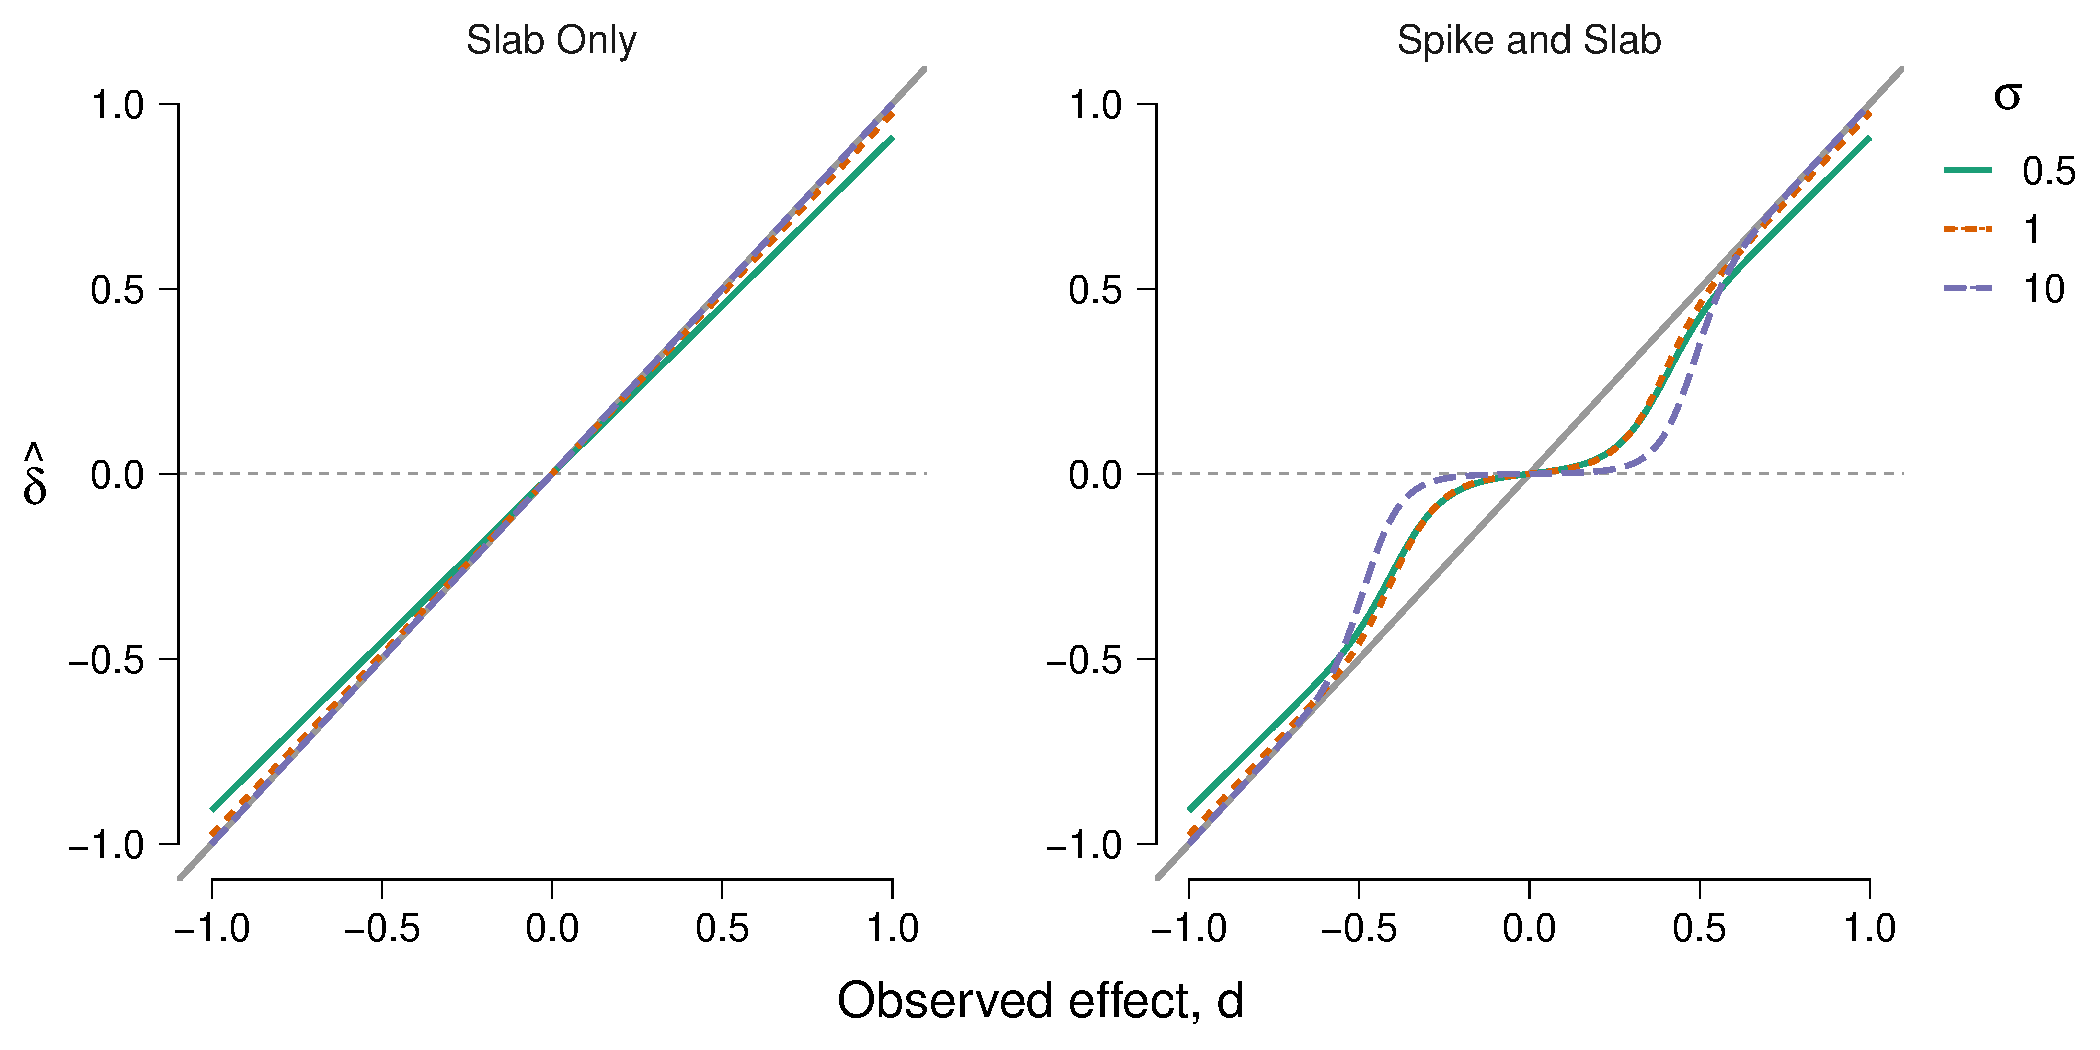
\includegraphics[width=\textwidth]{posteriorMeanVsSampleDelta_sigma_n_40.pdf}
%	\caption{%
%		Observed effect versus posterior mean for inference based on the slab only (left panel) and inference based on the spike-and-slab model (right panel).
%		Different lines represent different standard deviations for the prior distribution on $\delta$.
%		The sample size was 40 for both panels and the prior probability of the spike was $\nicefrac{1}{2}$.
%	}
%	\label{fig:S_vs_SS40}
%\end{figure}
The shrinkage can be explained in the following way.
Whenever the observed effect size is small, the data are well described by an effect size of 0 and thus the posterior probability of the spike is substantial.
In contrast, when the observed effect size is large the data are poorly described by an effect size of 0 and the posterior probability of the spike is negligible.
As a consequence, the estimate of the spike-and-slab is practically equivalent to the estimate of the slab.
The plots in the right column of Figure~\ref{fig:S_vs_SS_4_panel} shows the effect of sample size on the shrinkage.
For the bottom right plot, $N = 100$, if the observed effect size is small then the estimate is still shrunken towards 0, but as the observed effect size grows the shrinkage decreases much more quickly than in the top right plot where $N = 40$.
This makes sense from a signal-detection perspective. 
If the observed effect size is, for example, 0.3 after 40 observations, the posterior probability of the spike is substantial.
However, after collecting 60 additional observations while the observed effect size remains 0.3, the posterior probability of the spike decreases as it becomes increasingly less probable that the data were generated with an effect size of 0.

%Figure~\ref{fig:S_vs_SS100} shows the exact same relation as Figure~\ref{fig:S_vs_SS40} but for 100 observations rather than 40.
%If the observed effect size is small then the estimate is still shrunken towards 0, but as the observed effect size grows the shrinkage decreases much more quickly than in Figure~\ref{fig:S_vs_SS40}.
%This makes sense from a signal-detection perspective. 
%If the observed effect size is, for example, 0.3 after 40 observations, the posterior probability of the spike is substantial, as indicated by the shrinkage in Figure~\ref{fig:S_vs_SS40}. 
%However, after collecting 60 additional observations while the observed effect size remains 0.3, the posterior probability of the spike decreases as it becomes increasingly less probable that the data were generated with an effect size of 0.
%\begin{figure}[!ht]
%	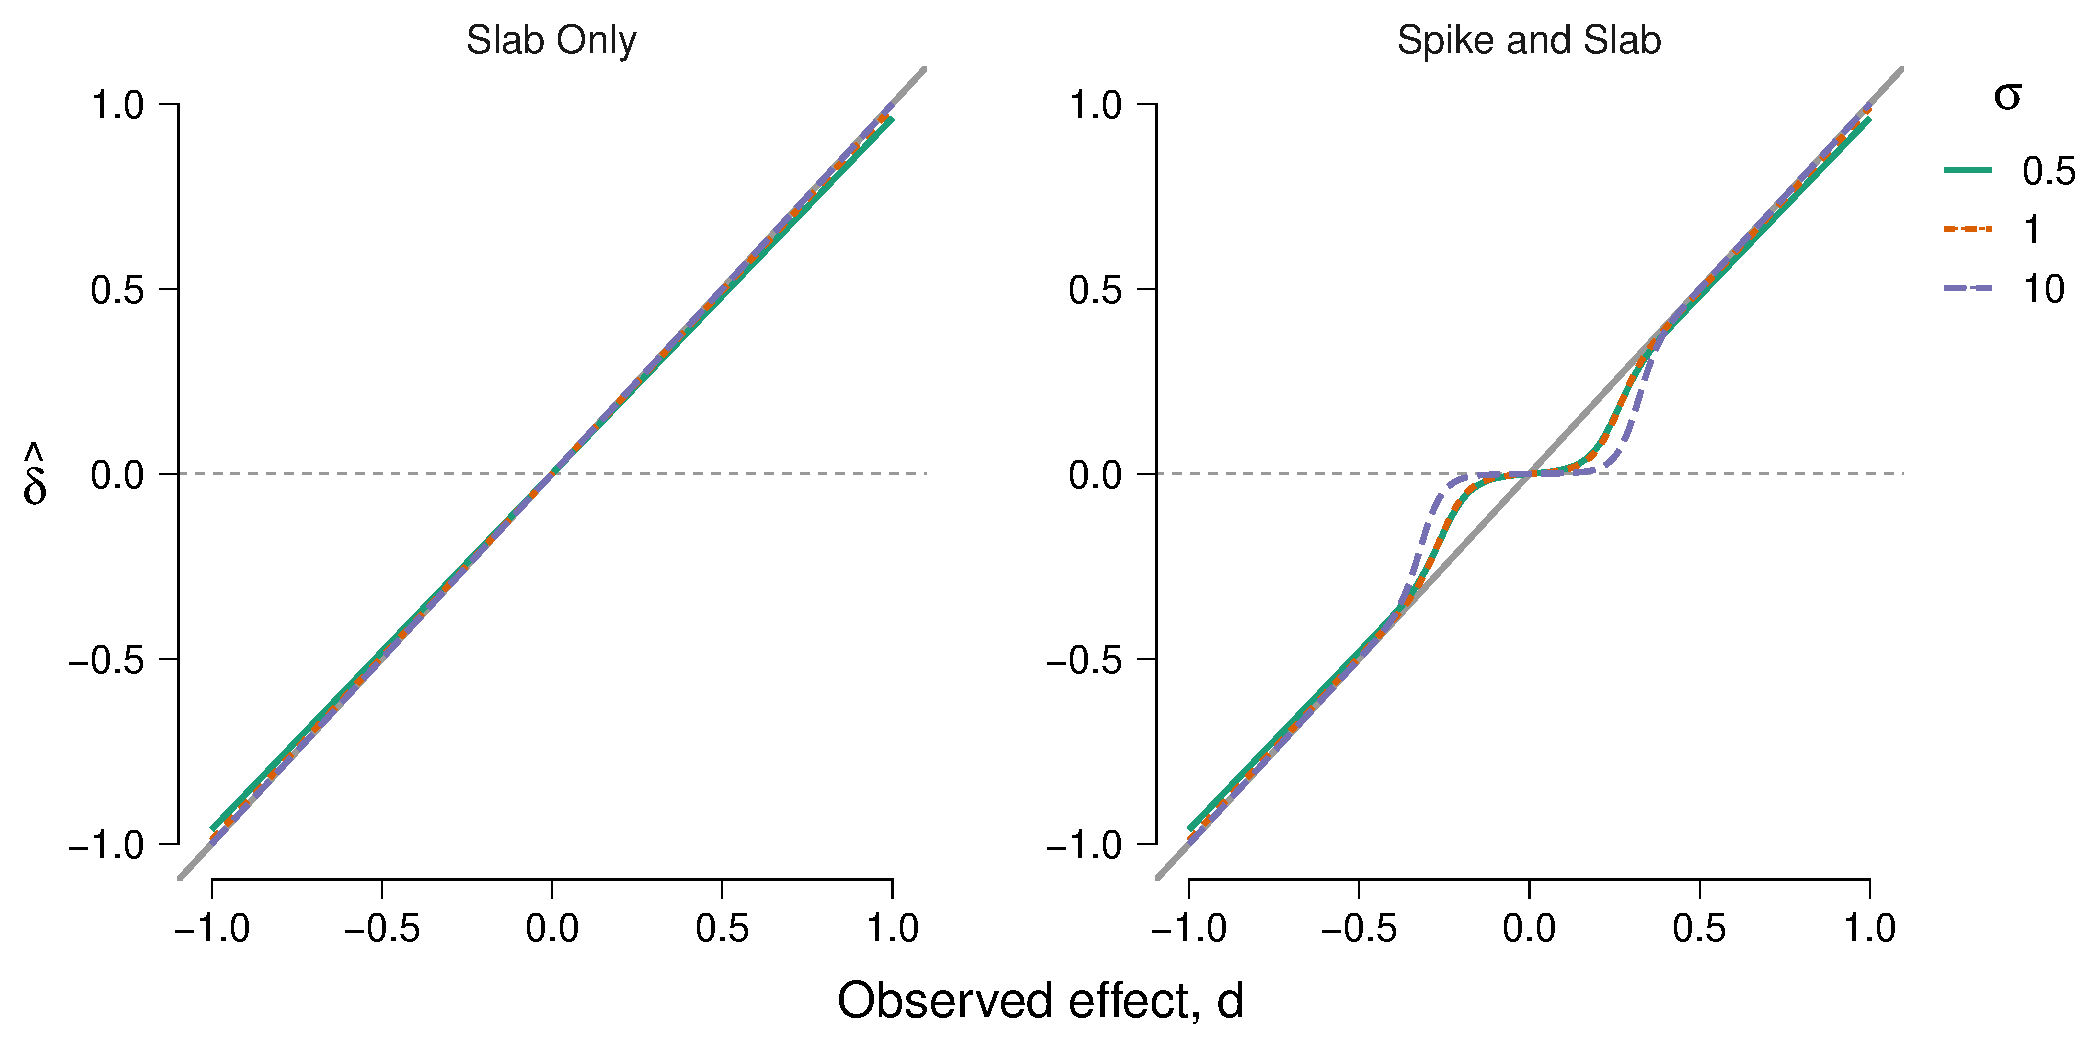
\includegraphics[width=\textwidth]{posteriorMeanVsSampleDelta_sigma_n_100.pdf}
%	\caption{%
%		Observed effect versus posterior mean for inference based on the slab only (left panel) and inference based on the spike-and-slab model (right panel).
%		Different lines represent different standard deviations for the prior distribution on $\delta$.
%		The sample size was 100 for both panels and the prior probability of the spike was $\nicefrac{1}{2}$.
%		\DON{Figures 3 and 4 could also be one four panel figure. Alternatively, Figures 3, 4 (right panel), and 5 could be one four panel figure.}
%	}
%	\label{fig:S_vs_SS100}
%\end{figure}
Next we explore the relation between shrinkage and the prior probability of the spike.
Figure~\ref{fig:S_vs_SS_PH0_40} shows the shrinkage for various prior probabilities.
The smaller the prior probability of the spike, the less the effect size is shrunken towards 0.
If the prior probability is small then the spike was a-priori implausible and less evidence is needed to make it's influence negligible.
\begin{figure}[!ht]
	\centering
	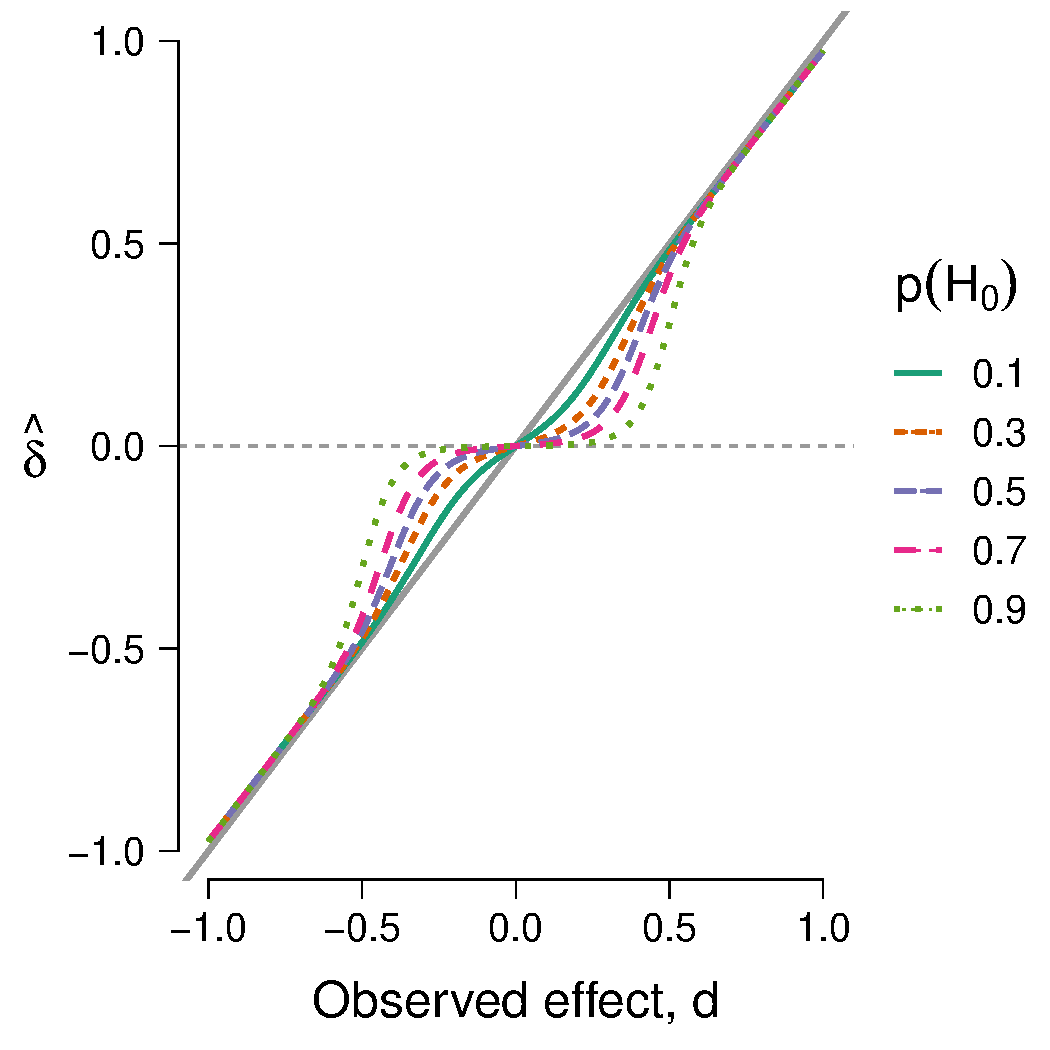
\includegraphics[width=.5\textwidth]{posteriorMeanVsSampleDelta_ph0_n_40.pdf}
	\caption{%
		Observed effect versus posterior mean (x-axis) versus the posterior mean of the spike-and-slab model (y-axis). The different lines represent different standard prior probabilities of the spike. The figure is based on 40 observations with a prior standard deviation of 1.
	}
	\label{fig:S_vs_SS_PH0_40}
\end{figure}

\section*{Empirical Example: Reanalysis of Two Minds}
\DON{I didn't get to including the results yet.}

To improve upon the previous fictional example, we highlight how the approach can be used in psychological practice by reanalyzing the results of \textcite{heycke2018two} using the spike-and-slab model.

%Here, we reanalyze the results of \textcite{heycke2018two} using the spike-and-slab model.
\textcite{heycke2018two} conducted two registered replications of \textcite{rydell2006two}.
We first briefly explain the design of the study before reanalyzing the results.

Participants were briefly shown a positive or negative prime on a computer screen.
Afterward, participants were immediately shown an image of a person.
Next, several behavioral descriptions that were either negative or positive appeared underneath the image of the person.
Participants were asked to indicate whether the behavioral description was characteristic or uncharacteristic for the person shown.
There were 200 trials, 100 trials showed positive primes and 100 trials displayed negative primes.
Half of the participants were first shown a block of 100 trials with positive primes whereas the other half were first shown the block of trials with negative primes.
After the first block, the participants performed a set of attitude measures.
These measures consisted
In total, data of 51 participants was analyzed.
For a detailed description see the ``Procedure'' section in \textcite{heycke2018two}.
\DON{TODO: explain this in more detail.}

\textcite{heycke2018two} did the following analysis. First they 


Following from both single-propositional and dual-process theories, \textcite{heycke2018two} expected a higher rating of the person shown whenever the positive behavioral descriptions were shown than when negative behavioral descriptions were shown. Since half of the participants were first shown positive primes before negative primes, this was tested with an interaction between time of measurement and positive/ negative primes.

This was tested by comparing the explicit attitude measure at block 1 with that at block 2. 

Under both single-propositional and dual-process theories 
we would expect a more favorable explicit rating of the target stimulus (i.e., Bob) when
positive behavior was characteristic of him than when negative behavior was characteristic
of him (Rydell et al., 2006). We thus expect a significant difference between the results of
the explicit attitude measure at time 1 compared to time 2, in the direction described above.


\end{revision}

\section*{Discussion}
\DON{Maybe add that the spike-and-slab is an alternative to the false dichotomy of NHST}
Standard estimates of effect size ignore the null hypothesis and are therefore overconfident, that is, biased away from zero. The spike-and-slab model remedies this problem by explicitly considering the possibility that an effect is absent \parencite{Robinson2019,RouderEtAl2018PBR}. The core idea dates back to \textcite{Jeffreys1939}; nonetheless, it is ignored both in empirical practice, in statistical education, and in journal guidelines.


%\subsubsection*{Extending the Null to a Perinull}
\subsubsection*{What if All Null Hypotheses Are False?}
The spike-and-slab approach clashes with the popular estimation mindset, where it is argued that statistical significance should be abandoned in favor of estimation \parencite{McShane2019abandon, Cumming2016introduction, valentine2015life, Cumming2014}. One argument to forgo hypothesis testing is that all null hypotheses are false \parencite{Cohen1990, Meehl1978} and therefore there is no need to consider a component that states that an effect is exactly zero. The statistical counterargument is that, even if point null hypotheses are false, they are still mathematically convenient approximations to more complex perinull hypotheses that allow mass on an interval close to zero \parencite{BergerDelampady1987, KiersTendeiro2019}. Thus, from a pragmatic perspective it is irrelevant whether or not null hypotheses are exactly true: in the spike-and-slab model, a perinull ``stake'' or ``chimney'' \parencite{KiersTendeiro2019} component will shrink estimates towards zero almost as much as the point null spike component will. 

\subsubsection*{When to Ignore the Spike}
There are two scenarios in which the presence of the spike (or perinull stake) can safely be ignored. First, the spike may be deeply implausible. This happens most often in problems of pure estimation, such as when determining the relative popularity of two politicians or the proportion of Japanese cars on the streets of New York. In such cases, no value or interval needs to be singled out for special attention. Second, the data may provide overwhelming evidence that an effect is present. When this happens, the results from a spike-and-slab model become virtually identical to those of a slab-only model, and the inclusion of the spike does not offer an added benefit. A practical recommendation by Harold Jeffreys is to ignore the spike whenever sample sizes fall between 50 and 2000 and the maximum likelihood estimate deviates from the spike by more than three standard errors (\cite[pp. 193--194]{Jeffreys1939}; \cite[p. 75]{Jeffreys1980}).



\subsubsection*{Conclusion}
Standard methods for estimating effect size produce results that are overly optimistic. This bias toward high estimates can be corrected by applying the spike-and-slab model which explicitly accounts for the possibility that the effect is absent. 

\newpage
\begin{NewBox2}[label=box:box1]{The Spike-and-Slab Distribution as Bayesian Model Averaging}{}%
	\vspace{6pt}\hrule\vspace{6pt}
	The spike-and-slab distribution can be viewed as a single model that consists of two components: the slab, which assumes that the effect is present, and the spike, which assumes the effect is absent.
	However, the spike-and-slab distribution can also be seen as a form of Bayesian model averaging.
	From that perspective, the spike and the slab are two individual models.
	The slab represents the unconstrained model that freely estimates effect size, and the spike represents the constrained model where the effect size is fixed to zero.
	Next, the results for each model are weighted by the posterior model probabilities and averaged, so that inference can be made using results from both models simultaneously.
	Such averaging over models yields optimal predictive performance (\cite[p. 640--641]{ZellnerVandaele1975}, as described in \cite[p. 600--601]{ZellnerSiow1980}; \cite[p. 57]{Haldane1932}; \cite{IversonEtAl2010}; \cite{RouderEtAl2018PBR}), and conceptually similar ideas date back much further (\cite[p. 387]{WrinchJeffreys1921}; \cite{Jevons18741913}).
	Note that these two perspectives ---a two-component model or averaging of two models--- differ in semantics but are mathematically equivalent.
\end{NewBox2}


\newpage

%\bibliographystyle{apacite}
%\bibliography{referenties, referenties.bib}
\printbibliography


\appendix
\begin{revision}%

\section*{Appendix}

\begin{figure}[!ht]
	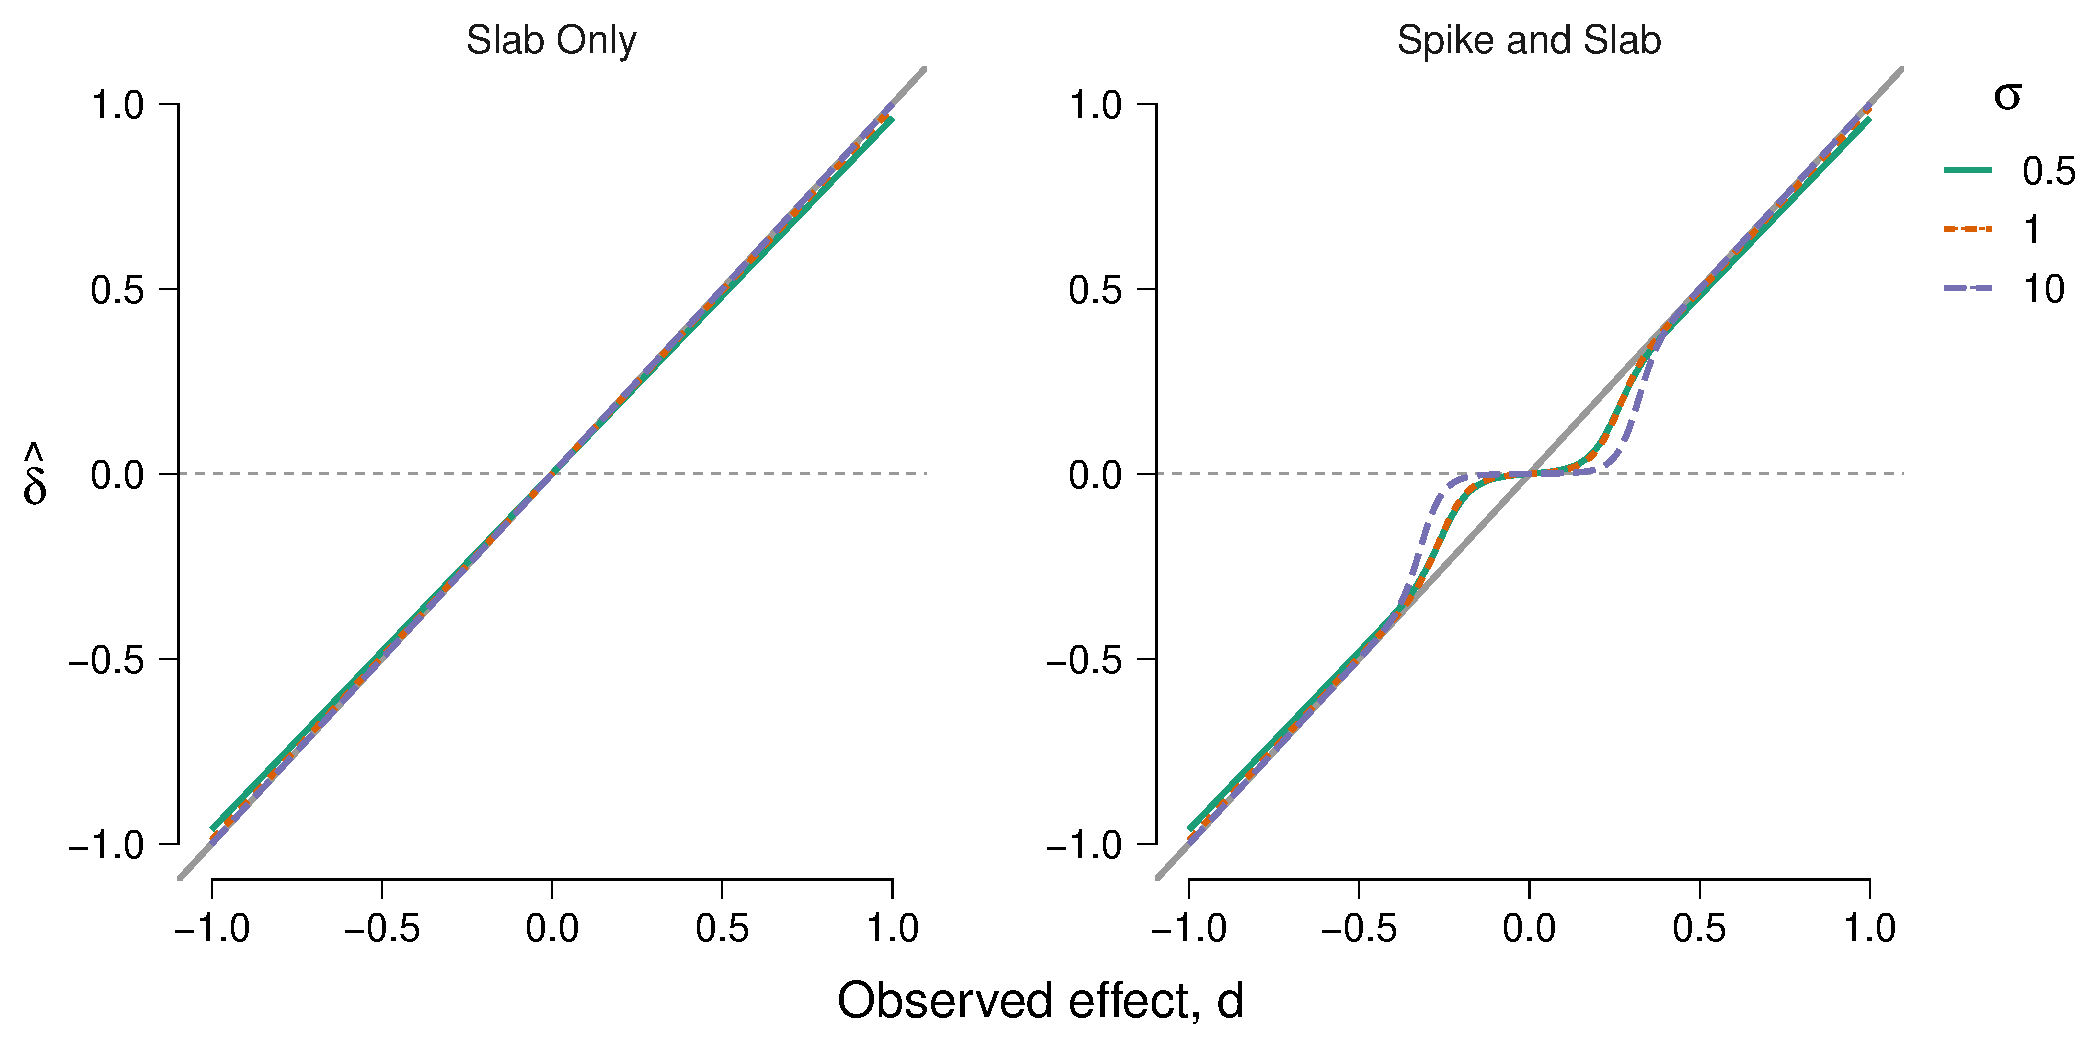
\includegraphics[width=\textwidth]{posteriorMeanVsSampleDelta_sigma_n_100.pdf}
\end{figure}
\end{revision}

\end{document}